\chapter{Datacenter}
10 years ago datacenters were no more than a room with some computers, air conditioners and some plugs to power up the devices.
Later on, customers started asking server vendors to include in the servers utilities to allow an \textit{automated datacenter management}.
Thus the trend moved towards \textbf{\ul{Software Defined Datacenter}}, which currently is the only possible way to deploy a Datacenter.
This refers to the fact that the behavior of some physical facility or system is not predefined in it’s building, but
to some extent it’s behavior is defined by a software and so it can be changed
over time, allowing for datacenters to be \textbf{future-proof}: servers may be replaced, but updating a whole datacenter is at least a 1-year project.

Datacenters \textbf{active} systems that allow to host server storage and network.


\section{Structure}
\textit{Racks} are made of ---$\sim 42$\footnote{for 2 meters tall racks}--- \textit{units}.
Racks are typically prefabricated in groups and automatically integrated in the datacenter POD (Point Of Delivery).\\
\note{Servers occupying only one rack unit are often referred to as Pizza Box}

Besides server theirselves, there is a \textbf{cooling system}.
The first issue is the how to provide cool air. Then there is also how to define an evacuation plan, which must take into account dust.

However also the \textbf{floor} is not to be negliged.
\begin{itemize}
   \item \textit{Floating} floor or Ground floor
   \begin{itemize}
      \item 
      \note{
         \textit{``A “floating floor” in a data center, also known as a “raised floor”, is a type of construction used in data centers to create a void between the actual concrete floor and the floor tiles where the servers and other equipment are located12. This space is typically used for routing cables and for air circulation, which helps with cooling the equipment1."}\footnote{ChatGPT 4.0 - Generated}
      }
   \end{itemize}
   \item \textit{Resistance} usually around $1 \frac{ton}{m^2}$  for marble tiles, about the half for wooden ones.
   \item \ul{Floating floors are always a good idea}.\\
   They provide flexibility, allow to have some sort of cable management under the racks, and in general make possible changing the layout without having to redo everything.
   \note{When the ceiling is not sufficiently high and no floating floor is possible, the cabling is done over the servers, which is not ideal.}
\end{itemize}

For example, in San Piero A Grado, there was a power cabin receiveing current from three lines.
Now the whole power management components are in a container outside the building placed close to the facility.

Cables are not super-resistant to current. A lot of current passing through a copper wire will \textit{exhaust} both the wire and the components receiving such current;
hence the current should also be balanced among different cables, to avoid exhausting some components before the others.


\ul{A \textbf{UPS}} ---first of all--- \ul{stabilizes the output current}.

In theory $1V * 1A = 1W$, but in reality, performing such conversion \ul{something gets lost}, so we have
\[I * V * cos \phi = W\]

\section{Power Management}

Electric panels (aka \textit{switchboards}) allow segmenting the power supply in the various zones of the datacenter.

\textbf{PDU}s stands for \textit{Power Distribution Units}, and allow to distribute power for a server units in a rack.
Typically, for each PDU there is another one, providing redundacy and thus resilience/robustness.

The UPS is attached to the PDU (Power Distribution Unit) which is linked to the server.
As briefly stated before ---for redundancy reasons--- a server is powered by a pair of lines, that usually are attached to two different PDUs. The server uses both the lines, so that there will be continuity in case of failure of a line. 
In the server there are the power plugs in a row that can monitored via a web server running on the rack PDU.

\nl

\textit{Inside} the datacenter \textbf{Direct Current} (DC) is preferred, because a DC power architecture contains less components (hence less heat production, hence less energy loss), but the problem is that the power companies supply our buildings with \textbf{Alternating Current} (AC).
ment.\\
AC is more efficient for power companies to deliver, but when it hits the equipment’s transformers, it exhibits a characteristic known as reactance.
Reactance reduces the useful power (watts) available from the apparent power (volt-amperes).
\begin{definition}[Power factor]
The \textit{power factor} is the ratio between the real power and the apparent power.
\end{definition}

\note{
   Early UPSs had a 0.8 PF, but today the standard is 0.9 PF.
   A 100 kVA UPS would support only 0.8 kW of real power load.
}

\begin{definition}[PUE]
\textit{Power Usage Effectiveness} \textbf{PUE} measures the efficiency of a Datacenter.
\[PUE = \frac{
   \textit{Total energy}
}{\textit{ICT energy}}\]
\end{definition}
The \ul{reason for improving Datacenter design is to lower the PUE};
basically to save money, but also for ``green-environment'' concerns.

\begin{center}
   But \textit{\ul{when}} should PUE be measured?
\end{center}
The PUE in January is very different from the one in August, so generally it is calculated as the average of one year.

Note that a poorly designed datacenter placed in Siberia with $-20^{\circ}$ may have a lower PUE than a datacenter in Italy, for instance.\\
In particulare geographical zones with high temperature variations over the year (e.g. in Italy the temperature variates from 40 to 50 Celsius degrees), are strongly unrecommended to build datacenters in.
\ul{A counterintuitive example is the desert}, where the temperature is very high during the day and very low during the night, but in general the temperature over the year is \textbf{stable}; allowing for defining physical processes exploiting such stability.\\
Also the oceans have a very stable temperature; not on the surface, but deep down it is very stable.

\section{Cooling}
Cooling is critical since its the most important factor in determining the \textbf{PUE}. Today the standard is air based\footnote{Does not mean that water cannot be implied in the process}, but there are some experiments for water based cooling.
\note{e.g. in the Netherlands there is a datacenter which uses water from the sea to cool down the datacenter.\\
Prof. Cisternino displayed a Microsoft datacenter in the sea, which is cooled down by the sea itself.}
Not all chilling techniques are possible in all places, because the temperature of the water must be lower than the one of the air, and the air must be dry.

Note that racks are always placed back-to-back, because the front requires cool air, and the back outputs hot air.
\subsection{CRAC}
\begin{figure}[htbp]
   \centering
   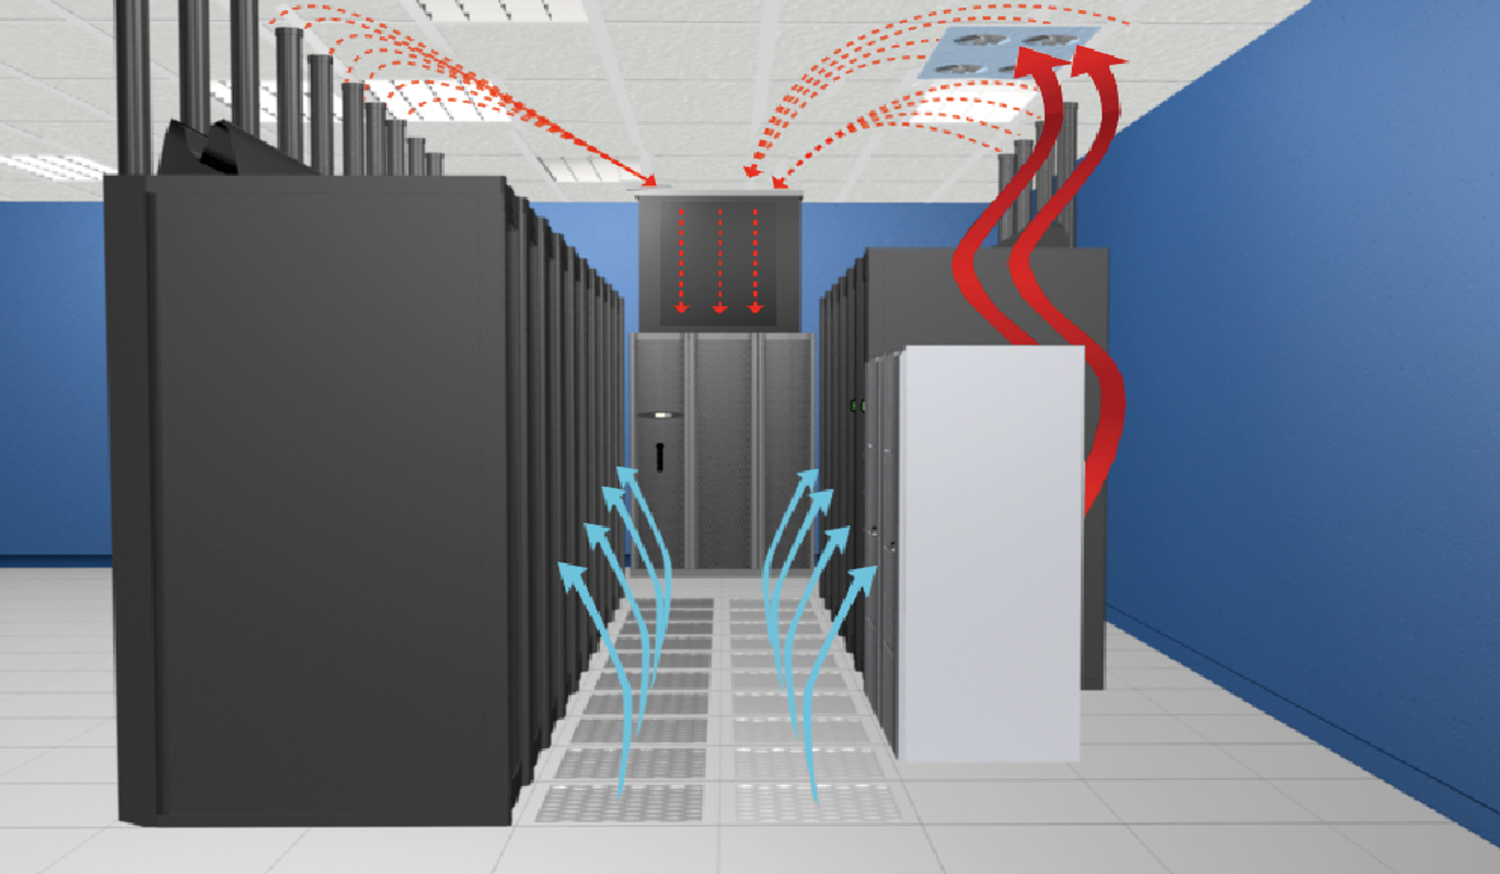
\includegraphics{images/CRAC.jpg}
   \caption{CRAC/CRAH cooling architecture}
   \label{fig:CRAC}
\end{figure}
Chillers take hot air from above and push cool air in the bottom. Then air pushed under the floating floor wants to exit, and does so going through the grates placed in front of the racks.
The racks suck the cool air in front and output hot air from the back.

{
   There are two \textbf{drawbacks}:
   \ns
\begin{enumerate}
   \item It is difficult to confine and keep separated hot air and cool air. The mixup between the two leads to cooling inefficiency, thus energy and money waste
   \item In case a rack has a workload heavier than others and thus requires more cooling air, the chiller must provide more cool air to all the racks in the same row;
   this makes this architecture particularly inefficient for datacenter which have heterogeneous workloads.
\end{enumerate}
}

No one is using this technique today apart from Aruba, since they have very omogeneus workload. Doors are used to isolate chilled and hot air.

\newpage
\subsection{Inrow Cooling}
\begin{paracol}{2}
   \colfill
   The fan ``towers'' are called \textit{inrow cooling}.

   The first advantage is that it allows for heterogeneous cooling in the datacenter.
   Secondarily, a fan outputs hot air directly where another fan expects it to be.
   This allows to confine hot air and to avoid wasting energy in outputting air and sucking it.

   \colfill
   \switchcolumn
\begin{figure}[htbp]
   \centering
   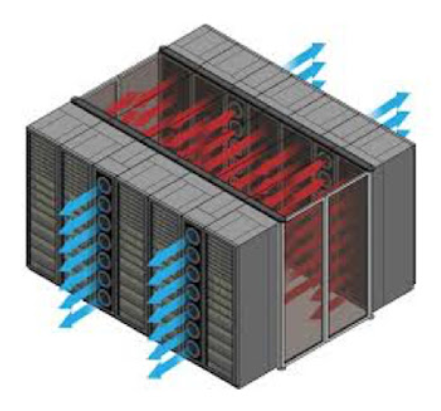
\includegraphics{images/inrow_cooling.png}
   \caption{Inrow cooling architecture}
   \label{fig:inrow_cooling}
\end{figure}
\end{paracol}

\subsection{Chilling water outside}

\begin{figure}[htbp]
   \centering
   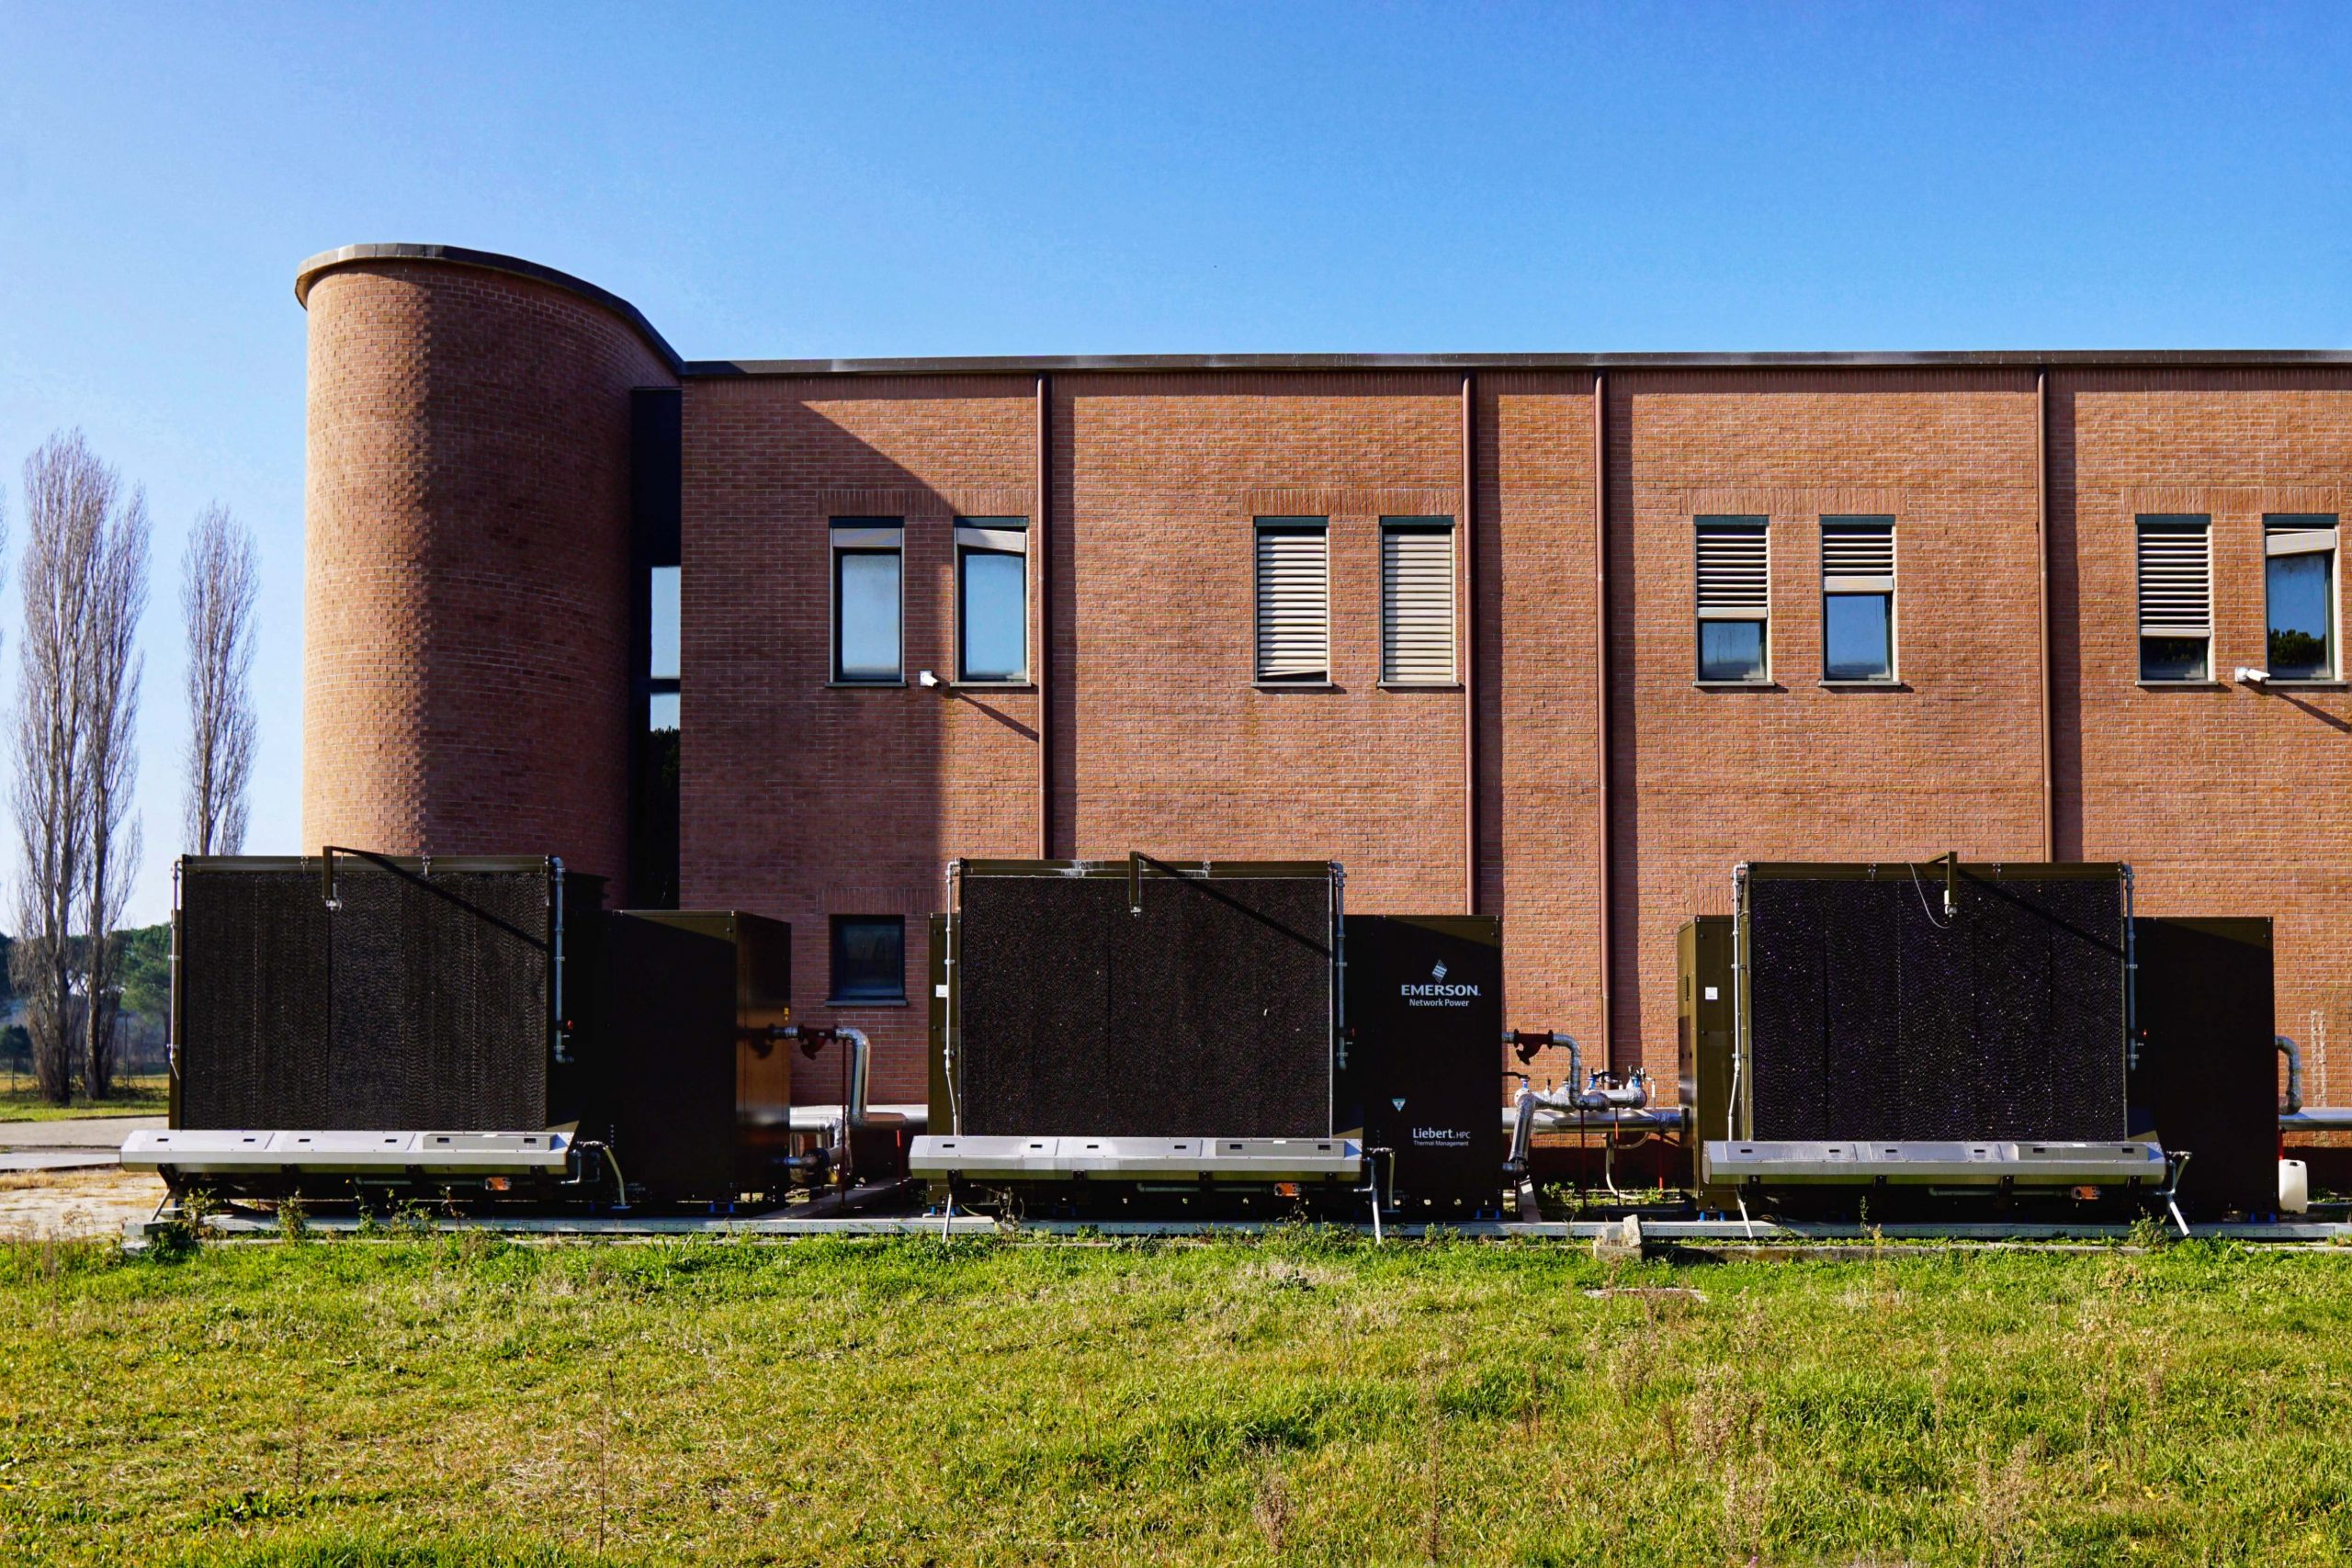
\includegraphics[width=0.45\columnwidth]{images/outside_chillers.jpeg}
   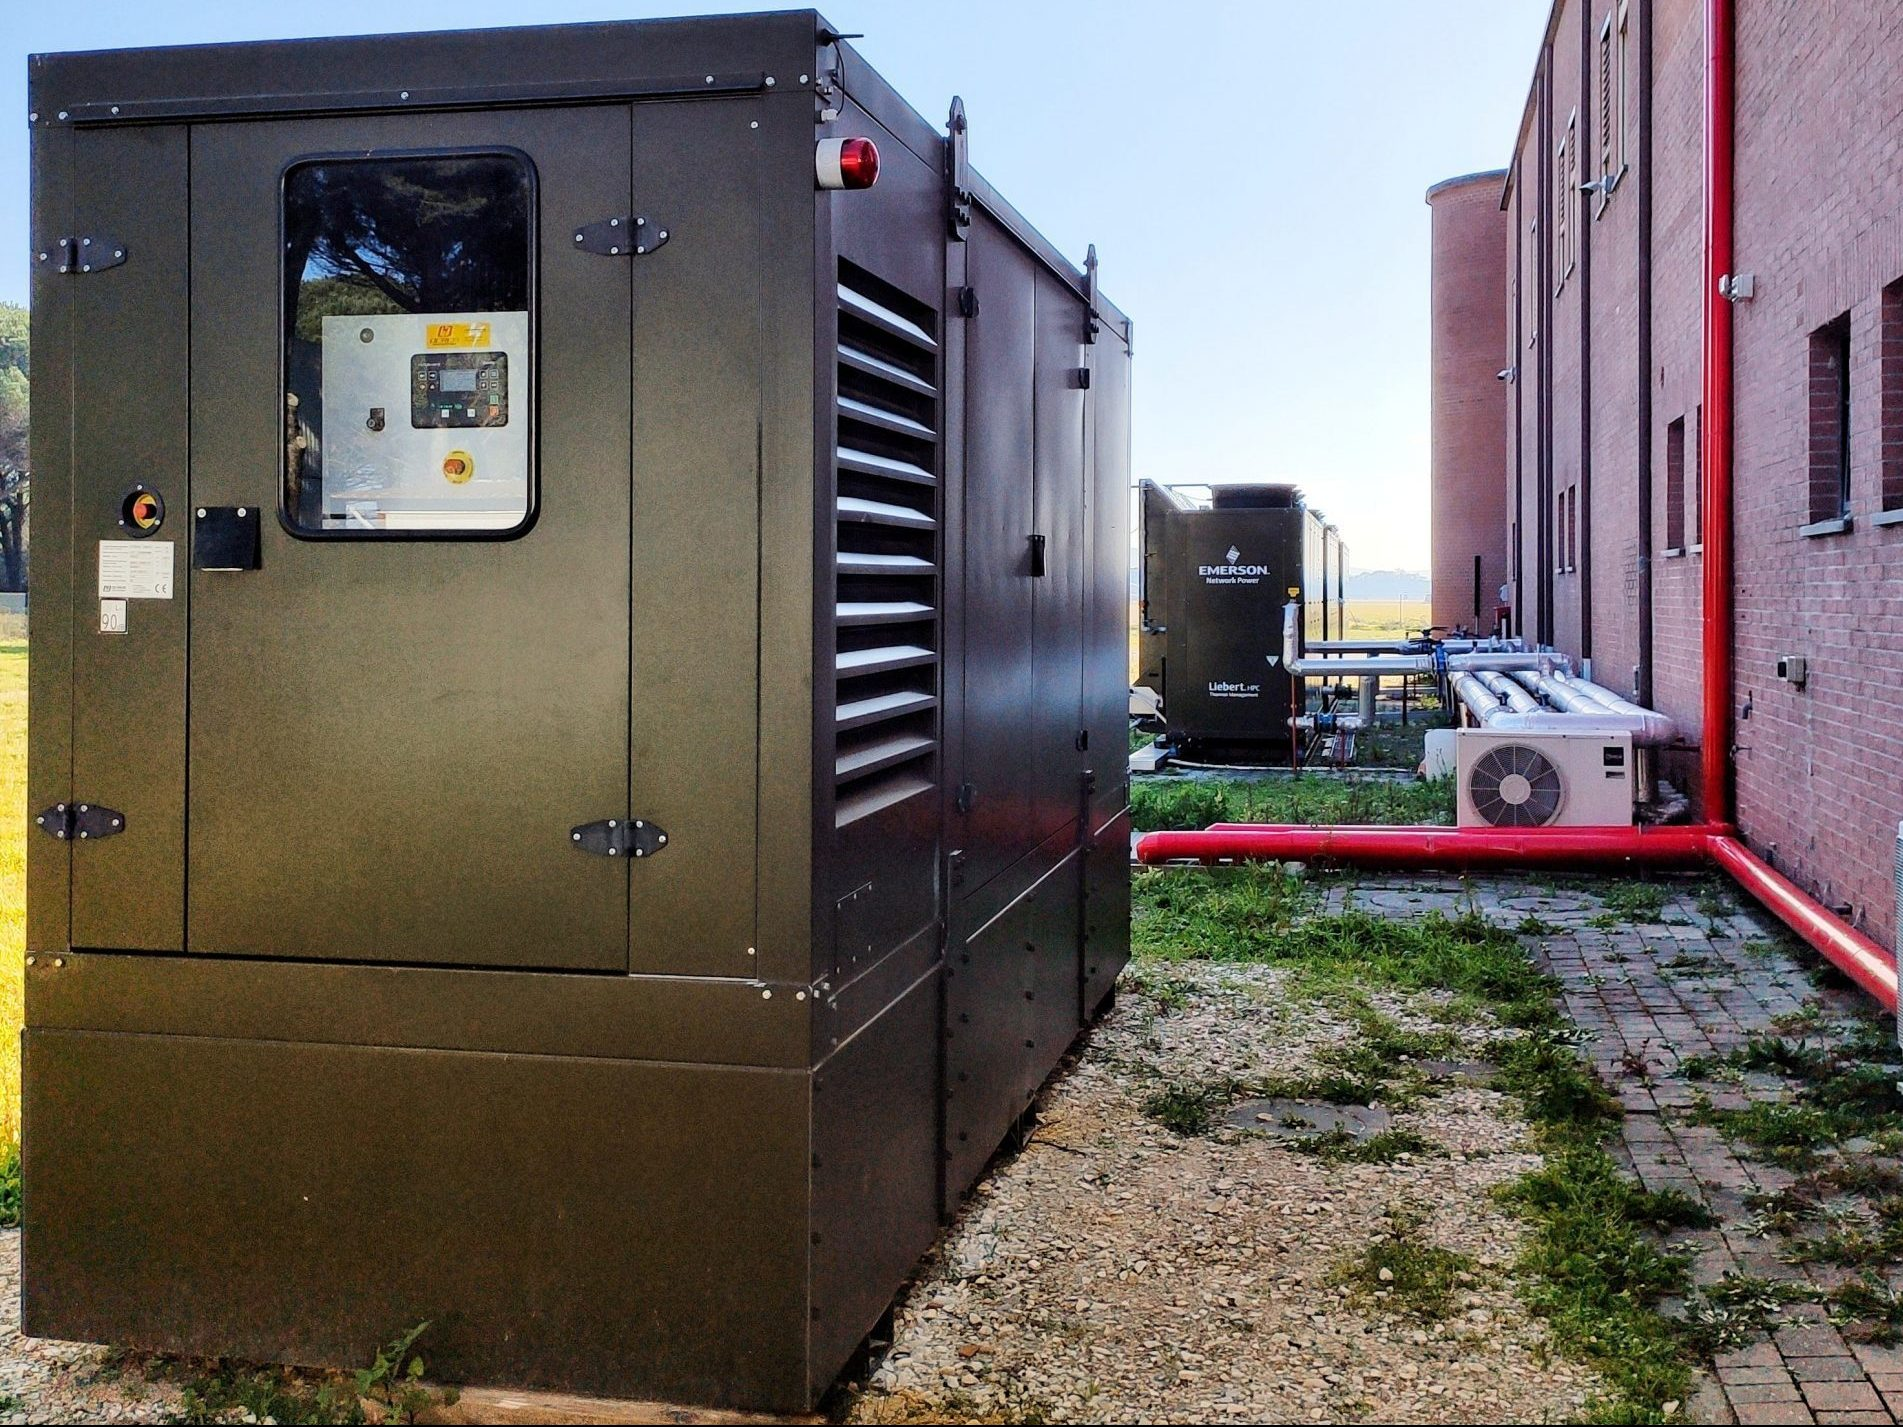
\includegraphics[width=0.405\columnwidth]{images/outside_chillers_2.jpeg}
   \caption{Outside chillers}
   \label{fig:outside_chillers}
\end{figure}
\textbf{Outside} of a datacenter there are chillers which cool down water which is then pumped into the datacenter, where it is used by CRAC/InRow chillers to cool down air.

It is important to ensure that the \ul{temperature does not heat up while travelling} from the outside chillers to the datacenter, because it would mean wasting energy. 

In SPG the outside chillers cool the water down to $18^{\circ}$, which \ul{seems high temperature, but in fact it is not}: the datacenter is designed to work up to $26^{\circ}$.
\begin{center}
   \ul{The higher the ``allowed'' temperature is, the more is the energy saved.}
\end{center}
Besides, \textbf{adiabatic} chillers ---such as the ones in SPG--- can use \textit{\textbf{free cooling}} in case the outside temperature is lower than $18^{\circ}$\footnote{common case in winter and autumn}, 
which basically exploits the lower outside temperature to \textit{passively} chill water, without involving the compressor used in the standard cooling way.
   
\nl

Also \textbf{humidity} must be managed. An environment which is too dry leads to water condensation onto racks and plugs, possibly resulting in damage to devices and humans.

\section{Redundancy for Resilience}
\textbf{Active-Passive} means that aside from the active system, there is a mirrored one which is shut down waiting for failure and boots up \textit{``just in case''}.
This approach is usually not the ideal one, because the second system is very unlikely to be used and is costful.
Besides, there are two critical issues with Active-Passive:
\labelitemize{\textit{Cons}}{
   \begin{enumerate}
      \item There is a non-negligible time interval where the switch from the active broken system and the passive one has to happen.
      \item If when booted the backup system reveals itself to be flawed and not working, well... \textit{very sad} \frownie
   \end{enumerate}
}

\textbf{Active-active} systems are usually better, because they also allow for load balancing. In case of SPG there are three cooling systems, and in case one breaks, the other two can keep working.
Active-active costs even more, but it is the standard way to go.

\section{Cooling CPU}
\begin{center}
   \ul{High-end CPUs \textit{heat up so much} that it has became \textit{unreasonable} to cool them using air.}
\end{center}

However, note that water conducts electricity, so a flaw in a waterpowered cooling system may lead to consistent damange and possible fires.

\textbf{Oil} instead doesn't conduct electricity, and there are some systems which are \textit{submerged} in oil, but there are two drawbacks:
\begin{enumerate}
   \item \textbf{Price}: oil is way more expensive than water
   \item \textbf{Servicing}: it is impossible to maintain the system's hardware.
\end{enumerate}

\textbf{Distilled water} is not conductive, but even not considering that distilling it is expensive, it is impossible to guarantee that is stays pure when travelling in pipes, chillers, and so on.

\nl

Most datacenters tend to have an hybrid approach to cooling, called \textbf{air-to-liquid}.
The idea is simple:
It is acceptable to use cool air to chill water, which is then used to chill the air by InRow coolers, which chills the liquid which chills the CPUs.
\note{(Woa! We need a schema...) }

\ul{This is \textit{not} the most efficient approach.}

A nice question would be, \textit{``Can't we simply chill the liquid and send it directly onto the CPUs?''} \textbf{No} \smiley.
\begin{itemize}
   \item Required pressure is different
   \item Required temperatures do not match
   \item Having water directly inside the datacenter is risky
\end{itemize}

\subsection{Spilling Pipes}
Liquid cooling systems manufacturers allow customers to ensure that their pipes are not spilling by injecting in the pipes a known gas at a known pressure.
The customer can measure the pressure when the product is shipped and check whether it is the expected one, and if not, send back the device.

\subsubsection*{Handling spills}
Handling spills is an \textbf{open problem}. 
Theorically, the idea would be to check for pressure variations, but this is \ul{currently \textit{impossible} to be done on each entrance of each rack.}
Too much actuaction and sensoring would be required.

Besides, in case a pipe is spilling, the operators must act \textit{quickly}, before the water spills onto other racks and cause critical damage. 

\subsection{Chassis}
\textbf{Chassis} are needed for various reasons:
\begin{itemize}
   \item 2.4GHz is the frequency at which water in our cells resonates, and circuits generate electromagnetic fields, so it may be unsafe to directly expose humans to circuitry
   \item Act as Faraday cages
   \item TODO
\end{itemize}